\section{Model Exercise 2-2 (03): Pressure driven percolation (healing)}
\label{sec:mex03}
%------------------------------------------------------------------------------
\Authors{Mathias Nest, Keita Yoshioka et al.}
%------------------------------------------------------------------------------
\subsection{Experimental set-up}
%------------------------------------------------------------------------------
One of the most important properties of barriers formed by salt or clay is their ability to close cracks and heal through creep. This means, that the materials can regenerate and regain their impermeability, after damage due to, e.g. excavation activities or  pressure driven percolation because of a temporary violation of the minimal stress criterion.

\begin{figure}[!ht]
\centering
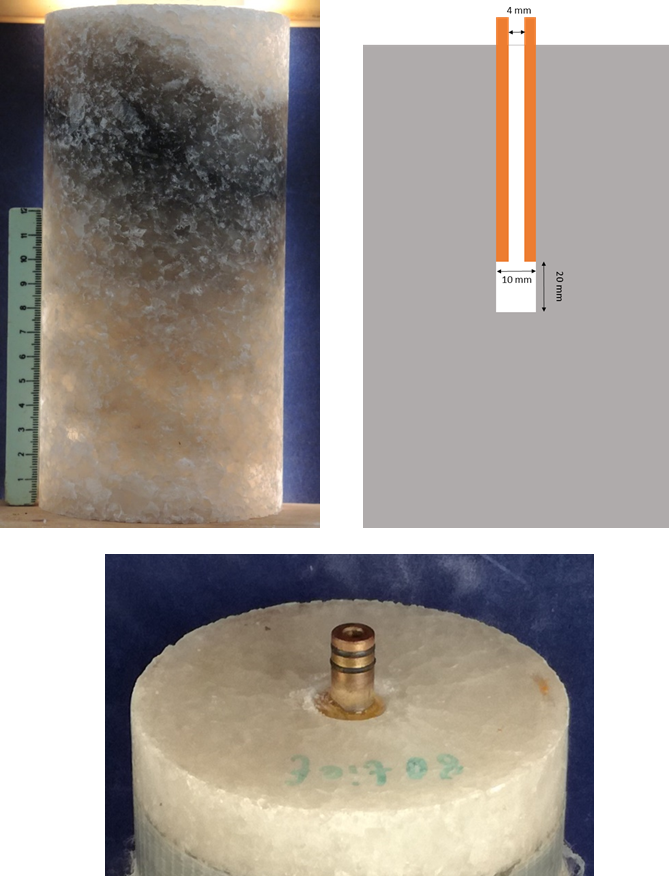
\includegraphics[width=8cm]{figures/mex3-exper-setup.png}
\caption{Rock salt sample, borehole geometry, detail of metal pipe.}
\label{fig:ME3-exper-setup}
\end{figure}

In this study we focus on the sealing of pathways and healing of cracks in salt and clay by measuring and simulating their gas permeability after damage has been done. 

For rock salt, we prepared cylindrical samples with a height of 20 cm and a diameter of 10 cm, with a borehole to the center, so that a gas pressure could be applied to a small area at the center. Initially all samples were placed under isostatic stress of 50 MPa for one day, to consolidate them. For the actual experiments the isostatic stresses were then changed to 10 MPa, 30 MPa, and 50 MPa, respectively. Before the gas pressure was applied, the plates which applied the axial stress were lock in place (''displacement boundary condition''). The gas pressure was increased in small steps, until a gas flow was detected. In all three cases a gas flow was detected before the percolation threshold was reached, which indicates that the samples suffered micro-fractures during preparation. After the last increase of the pressure, the flow rate was monitored for 24 to 70 hours under constant conditions.

\begin{figure}[!ht]
\centering
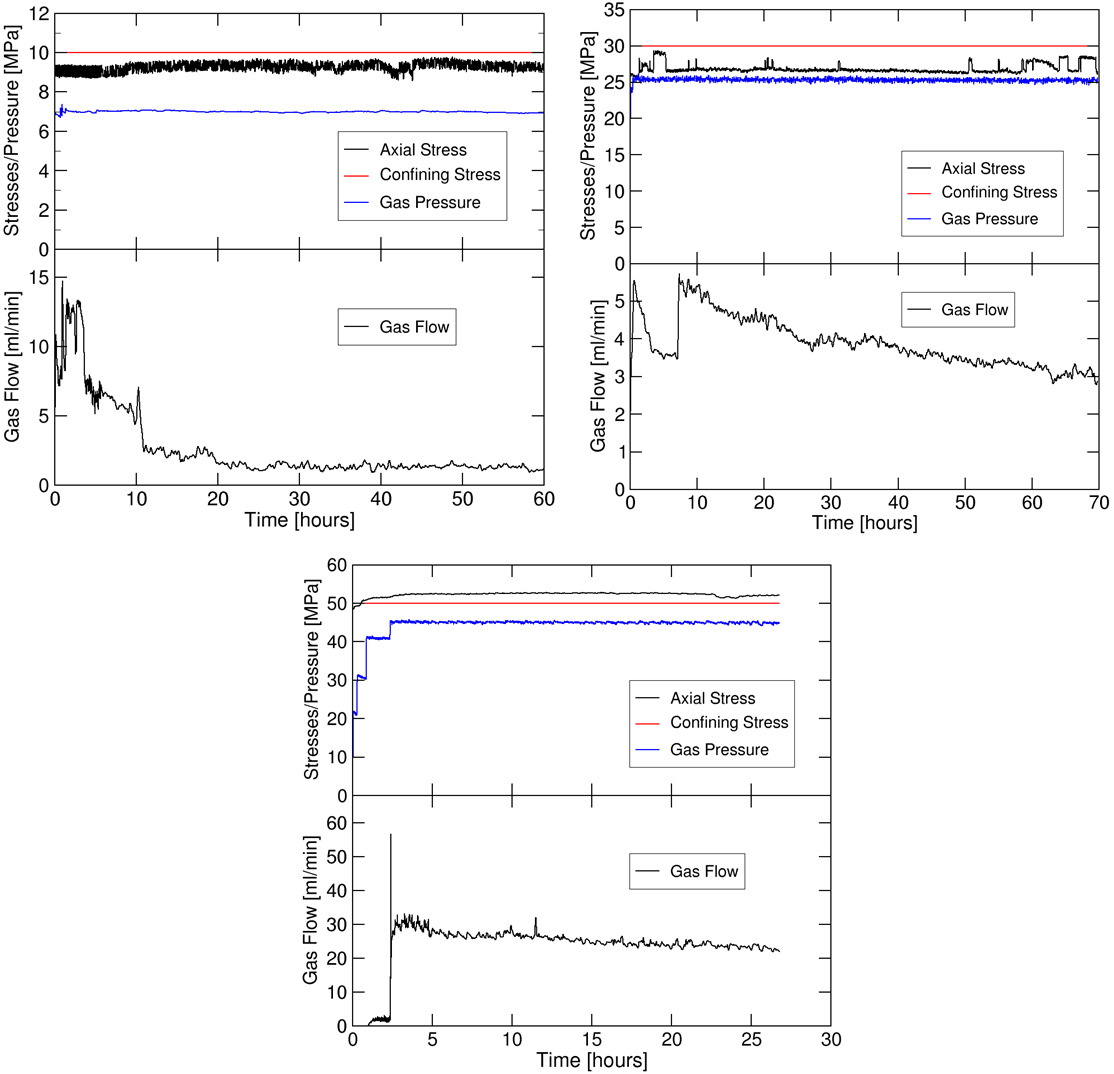
\includegraphics[width=1\textwidth]{figures/mex3-stresses-flows-v2.png}
\caption{Axial and confining stresses, gas pressures, and observed flow rates.}
\label{fig:ME3-stresses-flows}
\end{figure}
 
\begin{figure}[!ht]
\centering
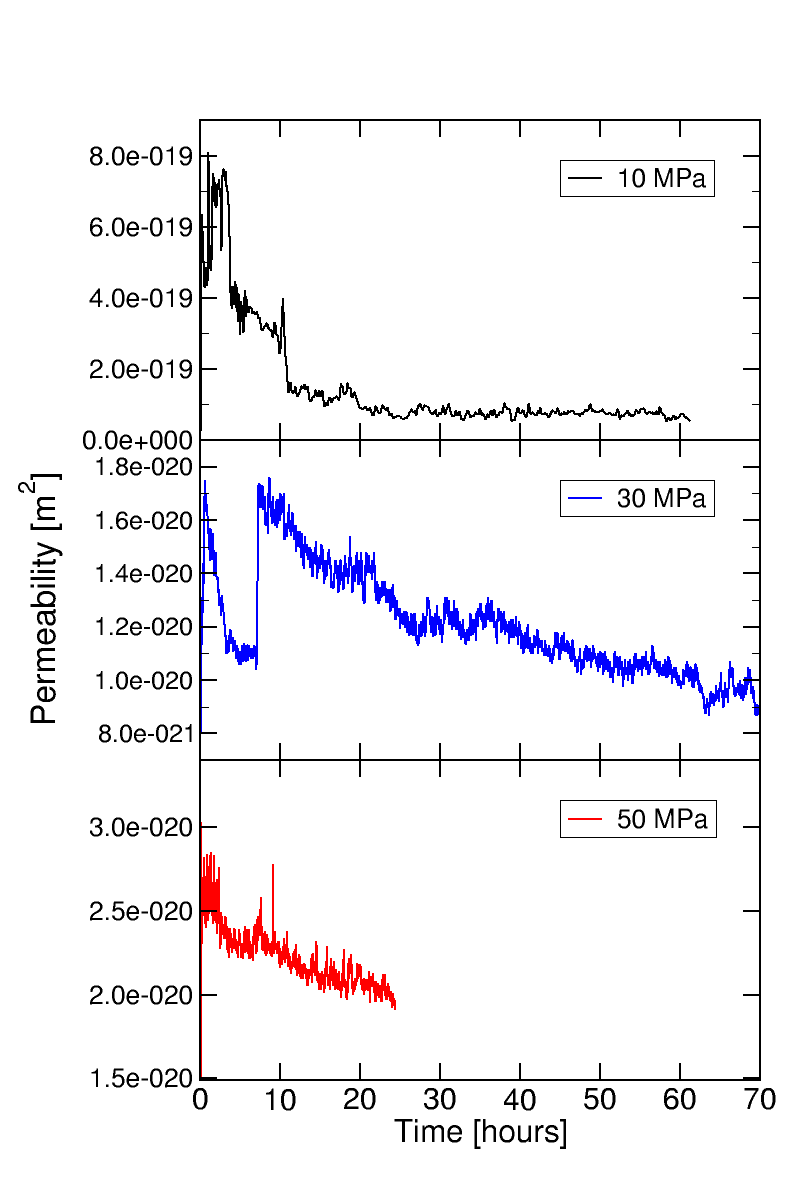
\includegraphics[width=9cm]{figures/mex3-perme-time-comparison.png}
\caption{Reduction of the permeability under different hydrostatic stress conditions.}
\label{fig:ME3-perme-exp}
\end{figure}

The flow rate can be converted into permeabilities, which are shown in Fig. \ref{fig:ME3-perme-exp}. For all three cases a reduction of the permeability is found,  showing that the cracks are narrowing and slowly closing. The abrupt and discontinuous manner of the change of the flow rate makes it difficult to identify time-scales of the processes involved. In the case of 10 MPa confining stress one can distinguish two phases. Between 3 and 24 hours after the start of the experiment, one can fit (admittedly only very crude) a time-scale of about 4.5 hours. Some larger pathways seem to close abruptly. After that, the pathways narrow only very slowly, presumably by creep processes, on a time-scale of about 1000 hours. In the cases of 30 MPa and 50 MPa we find time-scales of 30 hours and 11 hours, respectively. At least here, faster creep under higher stress is found as expected for the general trend.

\begin{figure}[!ht]
\centering
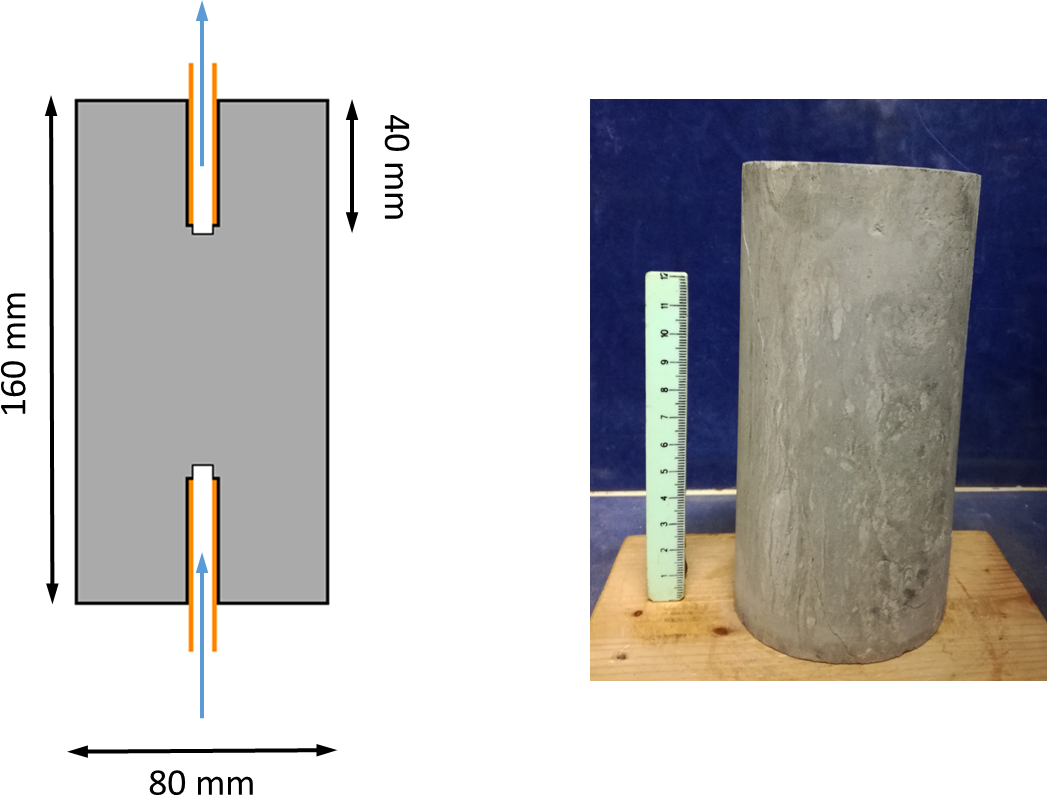
\includegraphics[width=9cm]{figures/mex3-claysample.png}
\caption{Left: Setup of the fracture closing experiment with Opalinus clay. Right: One of the samples.}
\label{fig:ME3-clay-setup}
\end{figure}

The Opalinus clay samples were prepared slightly differently, see Fig. \ref{fig:ME3-clay-setup}. The cylinders had a height of 160 mm and a diameter of 80 mm. Two boreholes were used, to avoid that under isostatic stress conditions the gas flows in a radial direction. Again it turned out, that the sample preparation had induced dilatant damage, so that a significant gas flow was already detected before the gas pressure reached the value of the mechanical stress. The subsequent results were obtained at a pressure of 0.5 bar. 

\begin{figure}[!ht]
\centering
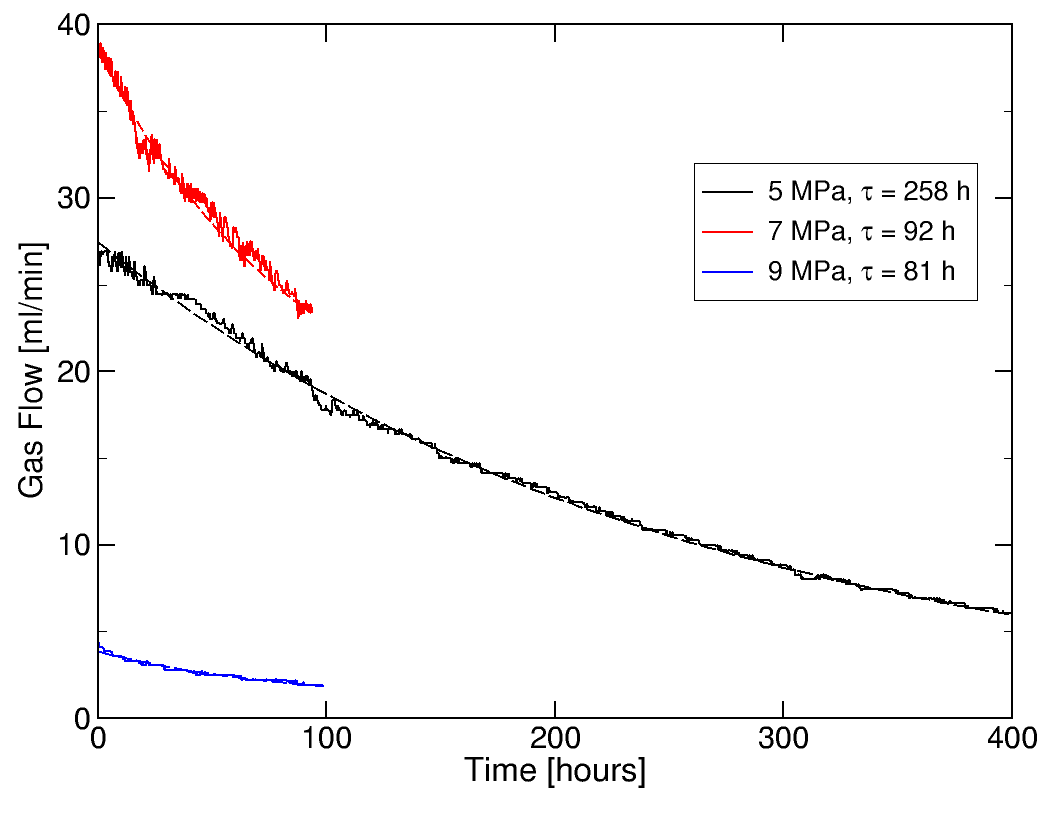
\includegraphics[width=9cm]{figures/mex3-senkrecht-alle.png}
\caption{Evolution of gas flow rates under different isostatic stresses.}
\label{fig:ME3-clay-flows}
\end{figure}

The results are shown in Fig. \ref{fig:ME3-clay-flows}. Initially, a stress of 7 MPa was applied, and the gas flow decreased from 38 ml/min to 24 ml/min in the course of about 100 hours. Then the stress was reduced to 5 MPa, which lead to an increased flow of 26 ml/min. Again, a decreasing rate was observed, reaching 6 ml/min after 400 hours. Finally the stress was increased to 9 MPa, and the rate dropped from 4.4 to 1.8 ml/min. So in all three cases the microfractures from the sample preperation were closing slowly, as a first step towards healing. The difference to the previous experiment with rock salt is stark. The clay reacted much more smoothly, and good fits to exponential decays could be obtained. The reason is the much smaller grain size in the clay, which permits much smaller displacements. In addition, the general trend, that the time scales decrease as the stresses are increased, is observed as expected. 

%------------------------------------------------------------------------------
\subsection{Model approaches}
%------------------------------------------------------------------------------
\subsubsection*{Discrete-Element-Model (DEM)}

The closure of cracks and the healing of rock salt after plastic deformation has been rarely looked upon and studied in detail. The purpose of this exercise is therefore to develop a phenomenological model, which can be incorporated into the 3DEC software. The mechanistic idea behind the process is shown in Fig. \ref{fig:ME3-crack-stre} Cracks have a rough surface, with high deviatoric stresses where they are in contact. This concentration of stress can lead to the abrupt abrasions observed above, and also to an increased creep rate. 

\begin{figure}[!ht]
\centering
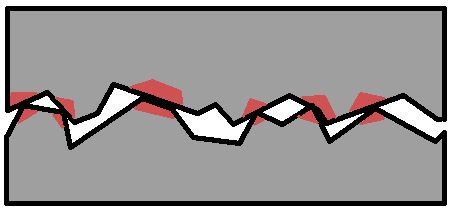
\includegraphics[width=8cm]{figures/mex3-crack-stresses.png}
\caption{Locations of high deviatoric stress in a crack. The deviatoric stress drives creep, which leads to a closing of the crack.}
\label{fig:ME3-crack-stre}
\end{figure}

In 3DEC the fluid flow is modelled using fluid knots, where apertures between two grains are defined. The size of the aperture depends on an elastic spring constant, the pressure, and two cut-off values, see Fig. \ref{fig:ME3-dem-apert}. There, $a_{max}$ and $a_{res}$ are the maximally and minimally allowed fluid apertures, and $a_0$ is the aperture when the normal stress $\sigma_N$ is equal to the fluid pressure $p$. In the following simulation we used $a_{res}$ = $a_0$ = 10$^{-7}$ m. The narrowing of the crack is then modelled by decreasing $a_{max}$ with time. 

\begin{figure}[!ht]
\centering
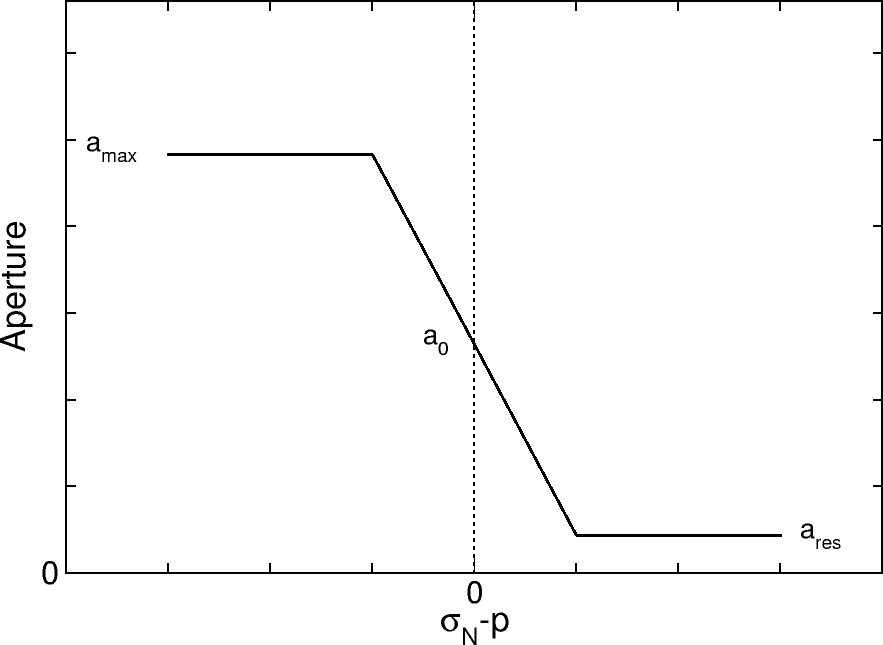
\includegraphics[width=8cm]{figures/mex3-aperture.png}
\caption{Schematic representation of the relation between aperture on grain boundaries and effective stress in 3DEC.}
\label{fig:ME3-dem-apert}
\end{figure}

The net effect of this approach is hard to predict, because the total fluid flow through the sample depends on a complex network of fluid knots with different orientations and normal stresses. Two approaches were tried: 

\begin{equation}
a_{max,n+1} = c \cdot a_{max,n} \quad \mbox{ with } 0<c<1
\end{equation}
and
\begin{equation}
a_{max,n+1} = a_{max,n} - \Delta a \quad .
\end{equation}

\begin{figure}[!ht]
\centering
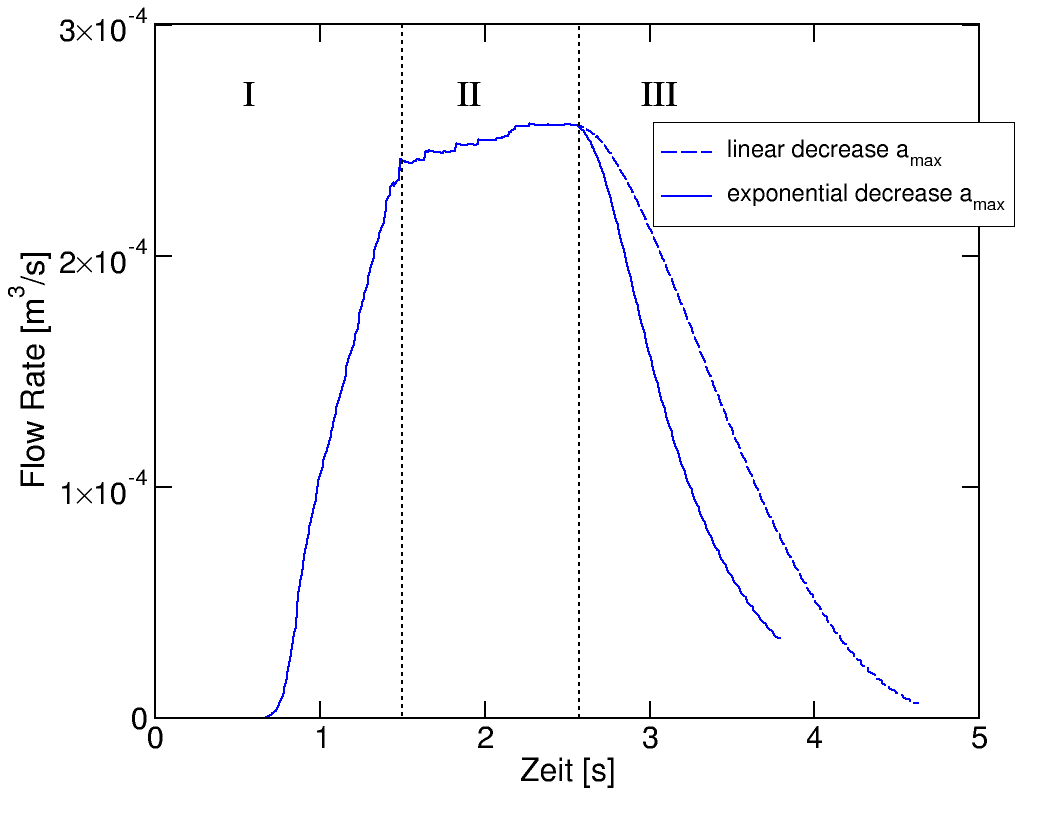
\includegraphics[width=8cm]{figures/mex3-flowrate-run3beide.png}
\caption{Pressure driven percolation and subsequent crack closure.}
\label{fig:ME3-flowrate-beide}
\end{figure}


The model setup used for this simulation was the same as in section \ref{sec:mex02}. The first two phases of the simulation agree with the simulation of the pressure driven percolation. A fluid pressure was applied to the internal cavity, and after a while liquid started to leak out (see phase I in Fig. \ref{fig:ME3-flowrate-beide}). After about 2.5 s the leak rate converged to a near constant level (phase II). From this point on, the simulation was run (phase III) in two different versions, corresponding to the two different equations above for the decrease of $a_{max}$. 

For the linear decrease of the maximum aperture we find a decrease of the flow rate that is not exponential as in the experiment (nor is it linear). For the exponential decrease we used $c$ = 0.9659 and applied this value every 100000th fluid timestep. (The full simulation required more than 10 million timesteps.) In this case a very good exponential fit with a time scale of 0.63 s could be obtained. It should be noted that in this simple setup, two time scales are actually mixed, which in reality are separated: In reality, creep (and thus the narrowing of the cracks) works much slower than the fluid dynamics. But as this exercise is a proof of concept, and serves to obtain a basic understanding of how how to model the phenomenon of crack closure, we accepted this approximation. 

\subsubsection*{Finite-Element-Model: Variational Phase-Field (VPF)}

\begin{figure}[!ht]
\begin{subfigure}[c]{0.49\textwidth}
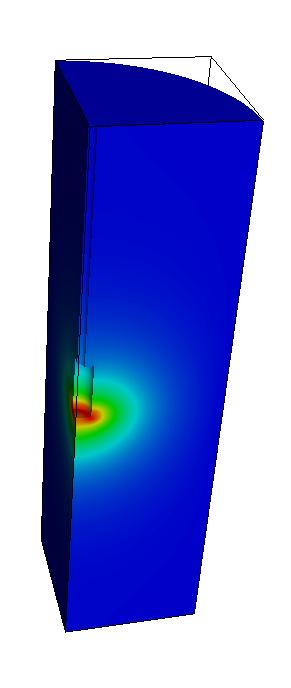
\includegraphics[width=1\textwidth]{figures/ME3_pres.png}
\subcaption{ME3 VPF model set up for the model exercise 3}
\label{fig:ME3_VPF_model}
\end{subfigure}
\hfill
\begin{subfigure}[c]{0.49\textwidth}
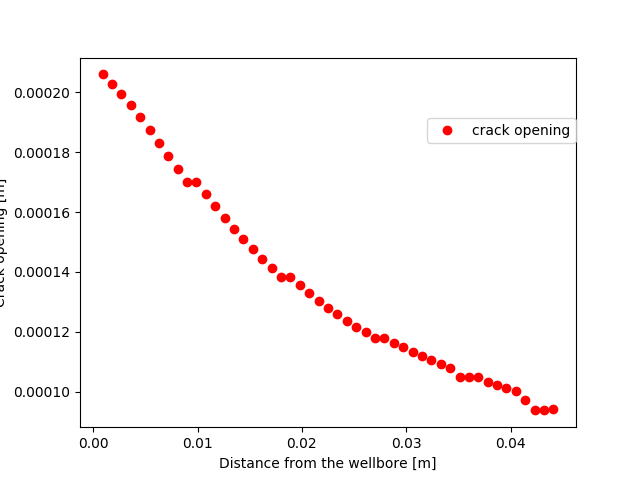
\includegraphics[width=1\textwidth]{figures/ME3_CrackWidth.png}
\subcaption{ME3 VPF crack width}
\label{fig:ME3_VPF_crack width}
\end{subfigure}
\caption{ME3 VPF preliminary}
\label{fig:VPF_ME2_creep}
\end{figure}

Implementation of the crack healing through creep model within the OGS variational phase-field model is being planned.
Crack opening (fracture width) is not a directly computed variable within the variational phase-field model, instead it is computed currently by taking a line integral~\cite{Yoshioka2020} as:
\begin{equation}
\left \llbracket \vec{u}\cdot \vec{n}_\Gamma \right\rrbracket
\approx \int_{l} \vec{u} \cdot \nabla v .
\label{eq:width_line_integral}
\end{equation}
where $l$ is the line that follows the normal direction to the crack $\Gamma$.
With a creep model, the displacement will be decomposed into the elastic $\vec{u}^e$ and the creep part $\vec{u}^c$ as $\vec{u} = \vec{u}^e+\vec{u}^c$, and the crack opening can be computed then by
\begin{equation}
\left \llbracket \vec{u}\cdot \vec{n}_\Gamma \right\rrbracket
\approx \int_{l} \vec{u}^e \cdot \nabla v .
\label{eq:width_line_integral}
\end{equation}
As $\vec{u}^c$ evolves with time, the crack opening will be subject to change and be able to simulate the aperture change observed in the experiments.
A preliminary attempt to calculate the fracture aperture from the elastic response only is shown in  Fig~\ref{fig:VPF_ME2_creep}.

%------------------------------------------------------------------------------
\subsection{Results and discussion}
%------------------------------------------------------------------------------
\todo[inline]{[UFZ] Please add results and discussion}
\todo[inline]{[UFZ] MEX 2-2 requires salt mechanics coupling and has not been done yet. It will follow once the MEX 2-b, 2-3, 3-3 are finished.}